\chapter{Integración del sistema en ROS 2}
\label{cap:capitulo6}

\section{Introducción}
\label{sec:segundaseccion}

Una vez validado el modelo cinemático del CDPR en todas las simulaciones mencionadas en el capítulo anterior, el siguiente paso consiste en la integración completa del sistema en ROS 2 \cite{ros2_docs}, lo que va a permitir dotar al sistema de una arquitectura modular y escalable, facilitando así su visualización a la hora de probarlo en un sistema físico real.

\vspace{0.25cm}

En este capítulo se describe la estructura general de los paquetes de ROS 2 \cite{ros2_docs} desarrollados, el funcionamiento del nodo que implementa toda la parte de control del CDPR, todo lo relacionado con las comunicaciones realizadas mediante topics y servicios, y la visualización del sistema en RViZ \cite{rviz_docs}.

\vspace{0.25cm}

Toda esta integración se ha llevado a cabo haciendo uso de la distribución Jazzy de ROS 2 \cite{ros2_docs} y de Python como lenguaje de programación, tal y como se mencionó en el capítulo anterior.

\newpage

\section{Estructura de los paquetes}
\label{sec:segundaseccion}

\begin{code}[h]
\begin{lstlisting}
src
|-- cdpr_2d
|   |-- cdpr_controller.py
|   |-- config (RViZ)
|   |-- description (URDF)
|   `-- robot_state_publisher.launch.py
|
|-- cdpr_figures
|   |-- figures_library.py
|   `-- figures_service.py
|
`-- cdpr_interfaces
    `-- DrawFigure.srv
\end{lstlisting}
\caption[Estructura del workspace ROS 2.]{Estructura del workspace ROS 2.}
\end{code}

Esta organización del workspace permite distinguir claramente de qué tareas se encarga cada uno de los paquetes que lo componen. \textit{cdpr\_2d} implementa el controlador principal del sistema y todos los ficheros necesarios para su simulación y validación en RViZ \cite{rviz_docs}, \textit{cdpr\_figures} contiene una librería que permite generar trayectorias asociadas a letras, números, polígonos y otras figuras geométricas, y por último, \textit{cdpr\_interfaces} define las interfaces de comunicación haciendo uso de servicios.

\vspace{0.25cm}

Por tanto, esta separación facilita el mantenimiento del código y hace que sea más sencillo añadir nuevas funcionalidades y componentes sin necesidad de tener que reestructurar todo el workspace.

\section{Arquitectura interna del nodo principal de control}
\label{sec:segundaseccion}

El sistema integrado en ROS 2 \cite{ros2_docs} tiene como núcleo el nodo \textit{cdpr\_controller}, encargado de recibir las posiciones objetivo por las que se quiere desplazar el efector final para así poder aplicarlas en el modelo cinemático desarrollado, con el objetivo de obtener todos los parámetros relacionados con los cables y las poleas del sistema.

\vspace{0.25cm}

El nodo se inicializa y se mantiene activo en todo momento para que pueda recibir todos los mensajes que contienen cada una de las posiciones objetivo, simplificando la integración y el análisis del sistema completo.

\begin{figure} [h!]
    \begin{center}
        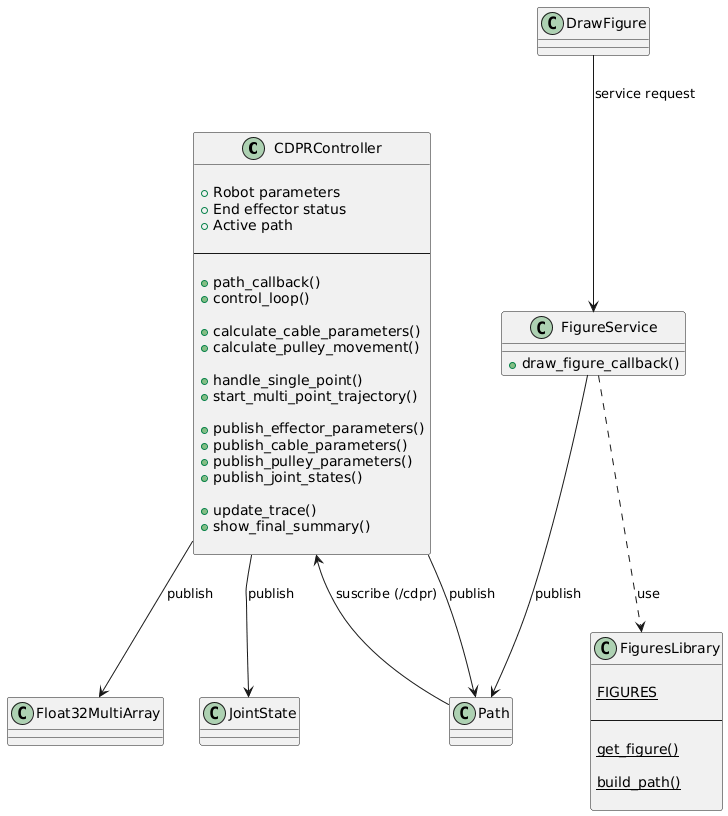
\includegraphics[width=\textwidth]{figs/class_diagram.png}
    \end{center}
    \caption{Diagrama UML de las clases que componen toda la arquitectura software desarrollada. En él se representan el controlador principal, el servicio encargado de generar figuras y la librería en la que se encuentran todas ellas predefinidas, además de las relaciones existentes entre todos los componentes mediante mensajes y servicios de ROS 2.}
\end{figure}\

Como se puede observar, la clase principal corresponde al nodo \textit{cdpr\_controller}, encargado de gestionar la ejecución del sistema dentro de ROS 2 \cite{ros2_docs}.

\newpage

Este nodo recibe todas las posiciones objetivo por las que se quiere desplazar el efector final haciendo uso del modelo cinemático para calcular todos los parámetros asociados a los cables y a las poleas, para posteriormente, publicar toda esta información en distintos topics.

\vspace{0.25cm}

Es por ello que esta organización es la que permite concentrar gran parte de la lógica del sistema en un único nodo principal, siguiendo una estructura que facilita la comprensión del mismo, y donde podrían llevarse a cabo ampliaciones en un futuro.

\vspace{0.25cm}

Para una mejor comprensión del comportamiento dinámico del sistema mostrado en la figura, se adjunta un enlace a un vídeo demostrativo al que se puede acceder haciendo clic \href{https://github.com/aleon2020/cable_driven_parallel_robot_2d/raw/refs/heads/main/media/gifs/3_or_more_points_execution.gif}{aquí}.

\begin{figure} [h!]
    \begin{center}
        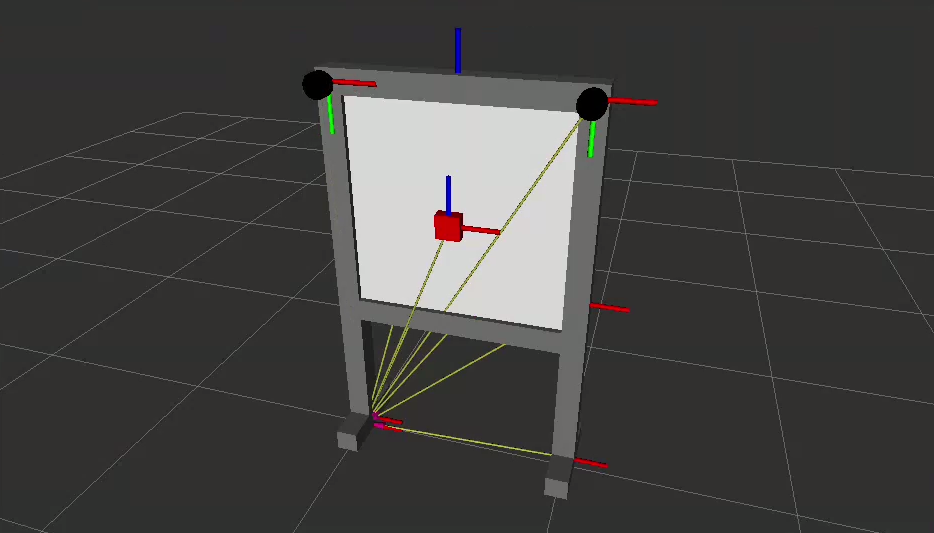
\includegraphics[width=\textwidth]{figs/cable_driven_parallel_robot.png}
    \end{center}
    \caption{Visualización en RViZ durante la ejecución de una trayectoria. En esta imagen se puede observar la estructura fija del CDPR en gris, el espacio de trabajo del efector final en blanco, las poleas en negro, y al propio efector final en rojo, mientras que en el vídeo adjunto se puede visualizar la evolución del movimiento del efector final y de las poleas conforme se actualiza el estado publicado por el nodo de control, lo que permite verificar si el comportamiento del sistema es correcto.}
\end{figure}\

\newpage

\section{Comunicación mediante topics}
\label{sec:segundaseccion}

La comunicación entre el nodo \textit{cdpr\_controller} y el resto del sistema se lleva a cabo utilizando topics que siguen un modelo publicador-suscriptor, lo que permite diferenciar los distintos componentes del sistema y monitorear el estado del mismo en tiempo real.

\vspace{0.25cm}

Por ello, se adjunta a continuación un diagrama de secuencia que muestra el intercambio de mensajes y cómo se produce esta comunicación entre los distintos componentes del sistema.

\begin{figure} [h!]
    \begin{center}
        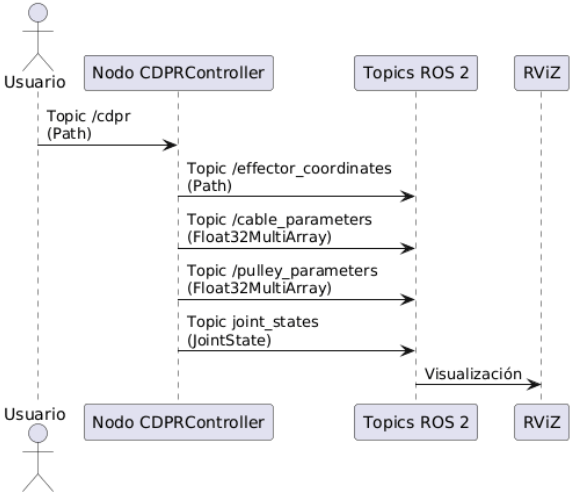
\includegraphics[width=\textwidth]{figs/communication_via_topics.png}
    \end{center}
    \caption{Grafo de comunicación que representa los nodos y topics utilizados durante la ejecución del sistema, donde se muestra el intercambio de información entre el controlador principal, los topics y las herramientas de visualización como lo es RViZ en este caso, facilitando así la comprensión del flujo de datos y las comunicaciones del sistema.}
\end{figure}\

\newpage

En primer lugar, el usuario publica una única posición o un conjunto de posiciones objetivo en el topic correspondiente. Después, el nodo \textit{cdpr\_controller} recibe este mensaje y va procesando cada una de las posiciones objetivo que ha recibido haciendo uso del modelo cinemático. Y por último, el nodo \textit{cdpr\_controller} publica en cada topic correspondiente mensajes sobre la posición del efector final o parámetros asociados a los cables y a las poleas, los cuales son también utilizados por RViZ \cite{rviz_docs} para poder representar el estado del sistema de forma visual y en tiempo real.

\section{Gestión de trayectorias y movimientos}
\label{sec:segundaseccion}

Además del paquete que contiene el nodo correspondiente al controlador principal (\textit{cdpr\_2d}), el sistema incluye un paquete llamado \textit{cdpr\_figures} que contiene una biblioteca de figuras predefinidas y se encarga de ofrecer servicios para su ejecución. Y por último, el paquete \textit{cdpr\_interfaces} define las interfaces de comunicación utilizadas como servicios personalizados. Es por ello que esta separación hace más sencilla la reutilización del código, resultando así en una arquitectura modular y escalable.

\vspace{0.25cm}

Este sistema tiene implementados diferentes modos de comportamiento en función del número de puntos recibidos en el mensaje de tipo \textit{nav\_msgs/msg/Path} \cite{nav_msgs_path}.

\vspace{0.25cm}

Cuando se recibe una única posición, el sistema interpreta la posición recibida como un posicionamiento fijo del efector final. En caso de haber recibido dos posiciones, se genera un desplazamiento entre una posición inicial y una posición final. Y por último, si se reciben tres o más posiciones, el sistema lo interpreta como una trayectoria compuesta por todas las posiciones que se le han pasado y por las que el efector final debe pasar en el orden especificado.

\vspace{0.25cm}

Para este último caso, el nodo interpola posiciones intermedias y aplica el modelo cinemático para calcular los parámetros correspondientes en todo momento para cada segmento de la trayectoria. Esto permite simular un movimiento contínuo y coherente del efector final dentro del espacio de trabajo.

\section{Visualización del sistema en RViZ}
\label{sec:segundaseccion}

La integración del sistema y su visualización en RViZ \cite{rviz_docs} son claves en el desarrollo del mismo, ya que permiten observar de forma mucho más clara el comportamiento del sistema. Para ello, se ha definido un modelo URDF \cite{urdf_docs} que describe la estructura fija, los cables, las poleas y el efector final.

\vspace{0.25cm}

El lanzamiento conjunto de los nodos \textit{cdpr\_controller} y \textit{robot\_state\_publisher} permiten actualizar en todo momento la visualización del robot en RViZ \cite{rviz_docs} según se va ejecutando cada trayectoria, cuya configuración facilita la observación de los distintos elementos que componen el sistema y su evolución cuando se encuentran en movimiento.

\section{Compilación y ejecución del sistema}
\label{sec:segundaseccion}

Con el objetivo de reproducir todo el trabajo desarrollado, se ha elaborado una \href{https://github.com/aleon2020/cable_driven_parallel_robot_2d/blob/main/README.md}{guía de ejecución} que enumera todos los pasos necesarios para compilar el workspace \cite{colcon_docs}, inicializar todos los nodos y poner en funcionamiento el sistema completo. Sin embargo, para no opacar la memoria con comandos u otras instrucciones de este tipo, dicha guía se incluye en el \href{https://github.com/aleon2020/cable_driven_parallel_robot_2d}{repositorio de GitHub oficial} de este proyecto.

\vspace{0.25cm}

La principal ventaja de trasladar toda esta información a un repositorio de GitHub \cite{github_docs,tfg_repository,microros_espidf,microxrce_dds} externo es que permite centrar la memoria en todos los aspectos relacionados con el diseño e implementación del sistema, además de proporcionar a quien la esté leyendo una referencia práctica para poder ejecutar todas las pruebas realizadas y utilizar el sistema completo desarrollado, facilitando así futuras modificaciones de los procesos de instalación y ejecución sin afectar a la estructura de la memoria.

\vspace{0.25cm}

Como inconveniente, la consulta de los pasos de instalación y ejecución del sistema requieren acceder a material externo a la memoria. Sin embargo, esta separación permite distinguir claramente entre la descripción técnica del sistema y las instrucciones necesarias para su ejecución.
